\documentclass[11pt]{article}
\usepackage{amsmath}
\usepackage{graphicx}
\usepackage{caption}
\usepackage{amssymb}
\usepackage{verbatim}
\usepackage{hyperref}
\usepackage{listings}
\usepackage{float}
\usepackage[thinc]{esdiff}
\usepackage{euscript}
\usepackage{subcaption}
\setlength{\parindent}{0em}
\newcommand*{\field}[1]{\mathbb{#1}}%
\usepackage{amsthm}
\newtheorem{claim}{Claim}
\captionsetup{labelformat=empty}

\begin{document}
\begin{titlepage} % Suppresses displaying the page number on the title page and the subsequent page counts as page 1
	
	\center % Centre everything on the page
	
	\vspace*{8cm}
	\vfill\vfill
	\textsc{Mathematical Tripos, Part 1B}\\
	\textsc{Computational project}
	\begin{center}
      {\huge\bfseries Ordinary Differential Equations\\[0.4cm]
}     \end{center}
	 % Title of your document
	
	\vfill
	
	
	
	
	%------------------------------------------------
	%	Date
	%------------------------------------------------
	\vspace*{\fill}
	\vfill\vfill\vfill % Position the date 3/4 down the remaining page
	
	{\large\today} % Date, change the \today to a set date if you want to be precise
	\vfill
	% Push the date up 1/4 of the remaining page	
\end{titlepage}
\section*{Question 1}
\begin{table}[!htb]
\centering
\caption{ h = 0.5}
\begin{tabular}{|c|c|c|c|c|}                
\hline                                      
 & $x_{n}$ & $Y_{n} $& $y_{e}(x_{n})$ & $E_{n}$\\                
\hline                                      
0 & 0.0000 & 0.0000 & 0.0000 & 0.0000 \\          
\hline                                            
1 & 0.5000 & 3.0000 & 0.3496 & 2.6504 \\          
\hline                                            
2 & 1.0000 & -14.8445 & 0.1350 & -14.9795 \\      
\hline                                            
3 & 1.5000 & 80.2799 & 0.0498 & 80.2301 \\        
\hline                                            
4 & 2.0000 & -431.0676 & 0.0183 & -431.0859 \\    
\hline                                            
5 & 2.5000 & 2315.9053 & 0.0067 & 2315.8986 \\    
\hline                                            
6 & 3.0000 & -12441.6589 & 0.0025 & -12441.6614 \\
\hline     
\end{tabular} 
\end{table}
      
\begin{table}[H]    
\centering   
\caption{ h = 0.375}
\begin{tabular}{|c|c|c|c|c|}              
\hline                                    
 & $x_{n}$ & $Y_{n} $& $y_{e}(x_{n})$ & $E_{n}$\\             
\hline                                    
0 & 0.0000 & 0.0000 & 0.0000 & 0.0000 \\          
\hline                                            
1 & 0.3750 & 2.2500 & 0.4226 & 1.8274 \\          
\hline                                            
2 & 0.7500 & -7.4058 & 0.2207 & -7.6264 \\        
\hline                                            
3 & 1.1250 & 29.5168 & 0.1053 & 29.4115 \\        
\hline                                            
4 & 1.5000 & -114.3128 & 0.0498 & -114.3626 \\    
\hline                                            
5 & 1.8750 & 444.4196 & 0.0235 & 444.3960 \\      
\hline                                            
6 & 2.2500 & -1726.9143 & 0.0111 & -1726.9254 \\  
\hline                                            
7 & 2.6250 & 6710.8405 & 0.0052 & 6710.8353 \\    
\hline                                            
8 & 3.0000 & -26078.3082 & 0.0025 & -26078.3107 \\
\hline                                                   
\end{tabular}                             
\end{table}

\begin{table}[!htb]
\centering
\caption{h = 0.25}                                     
\begin{tabular}{|c|c|c|c|c|}               
\hline                                     
 & $x_{n}$ & $Y_{n} $& $y_{e}(x_{n})$ & $E_{n}$\\               
\hline                                     
0 & 0.0000 & 0.0000 & 0.0000 & 0.0000 \\           
\hline                                             
2 & 0.5000 & -2.3853 & 0.3496 & -2.7349 \\         
\hline                                                                                        
4 & 1.0000 & -15.4461 & 0.1350 & -15.5811 \\       
\hline                                                                                          
6 & 1.5000 & -90.7083 & 0.0498 & -90.7581 \\       
\hline                                                                                      
8 & 2.0000 & -528.9572 & 0.0183 & -528.9756 \\         
\hline                                             
10 & 2.5000 & -3083.0916 & 0.0067 & -3083.0984 \\  
\hline                                                                                       
12 & 3.0000 & -17969.6134 & 0.0025 & -17969.6159 \\
\hline                                                
\end{tabular}                              
\end{table}

\begin{table}[H]
\centering
\caption{h = 0.125}                         
\begin{tabular}{|c|c|c|c|c|}              
\hline                                     
 & $x_{n}$ & $Y_{n} $& $y_{e}(x_{n})$ & $E_{n}$\\               
\hline                                     
0 & 0.0000 & 0.0000 & 0.0000 & 0.0000 \\   
\hline                                   
4 & 0.5000 & 0.0159 & 0.3496 & -0.3336 \\                                       
\hline                                     
8 & 1.0000 & -0.1781 & 0.1350 & -0.3131 \\ 
\hline                                                                      
12 & 1.5000 & -0.2620 & 0.0498 & -0.3118 \\
\hline                                                                      
16 & 2.0000 & -0.2937 & 0.0183 & -0.3120 \\
\hline                                                                       
20 & 2.5000 & -0.3054 & 0.0067 & -0.3121 \\
\hline                                                                      
24 & 3.0000 & -0.3097 & 0.0025 & -0.3122 \\
\hline                 
\end{tabular}                                                    
\end{table}  
                
\begin{table}[!htb]
\centering
        \caption{h = 0.1}                  
\begin{tabular}{|c|c|c|c|c|}            
\hline                                     
 & $x_{n}$ & $Y_{n} $& $y_{e}(x_{n})$ & $E_{n}$\\        
\hline                                     
0 & 0.0000 & 0.0000 & 0.0000 & 0.0000 \\  
\hline                                                                  
5 & 0.5000 & 0.3909 & 0.3496 & 0.0414 \\  
\hline                                    
10 & 1.0000 & 0.1223 & 0.1350 & -0.0127 \\
\hline                                   
15 & 1.5000 & 0.0528 & 0.0498 & 0.0030 \\ 
\hline                                                           
20 & 2.0000 & 0.0178 & 0.0183 & -0.0005 \\
\hline                                                               
25 & 2.5000 & 0.0069 & 0.0067 &1.786e-04 \\ 
\hline                                                                   
30 & 3.0000 &2.464e-03 & 2.479e-03 & -1.426e-05\\
\hline                                     
\end{tabular}                                   
\end{table}
    
\begin{table}[H]
\centering
\caption{h = 0.05}      
\begin{tabular}{|c|c|c|c|c|}               
\hline                                     
 & $x_{n}$ & $Y_{n} $& $y_{e}(x_{n})$ & $E_{n}$\\        
\hline                                     
0 & 0.0000 & 0.0000 & 0.0000 & 0.0000 \\  
\hline                                                                 
10 & 0.5000 & 0.3461 & 0.3496 & -3.4883e-03 \\
\hline                                                             
20 & 1.0000 & 0.13499 & 0.13500 & -9.6203e-06 \\
\hline                                                                
30 & 1.5000 & 0.049848 &0.049781 & 6.6688e-05 \\ 
\hline                                                                    
40 & 2.0000 & 0.018342  & 0.018316  & 2.6956e-05 \\ 
\hline                                                                  
50 & 2.5000 & 0.0067479 & 0.0067379 & 9.9924e-06 \\ 
\hline                                                                      
60 & 3.0000 & 0.0024824 & 0.0024788 & 3.689e-06 \\ 
\hline                                                                 
\end{tabular}                                            
\end{table}  
\pagebreak
The error oscillates wildly. If it grows proportional to $e^{\gamma x}$, then
$$\gamma = \frac{log(\mathopen|E_{6}\mathclose|)-log(\mathopen|E_{5}\mathclose|)}{3-2.5}  = 3.3625$$.
\\
The first column of each table is the index of point selected in all n points. In the above tables, I select points with the same values of x with the first table( except h = 0.375, where I preserved all outputs ), i.e. the table for h = 0.5. For h small enough, the numerical solution converges, and after the error starts to converge to 0, the instability decreases as h decreases.
\section*{Question 2}
\subsection*{(i) Analytic solution}
First solve homogeneous equation:
$$Y_{n+1} = Y_{n} + h[-12Y_{n}+4Y_{n-1}]$$
substitute:
$y = \lambda^{n}$,
obtain:\\
$${\lambda}_{1,2} = \frac{1-12h \pm \sqrt{(12h-1)^{2}+16h}}{2}$$
Therefore, the complementary function is:
$$Y_{n}^{(c)} = C_{1} {\lambda}_{1}^{n}+C_{2} {\lambda}_{2}^{n}$$
Then solve (Characteristic equation): \\
$$Y_{n+1} -Y_{n} +4h(3Y_{n} - Y_{n-1})=3h[3(e^{-2h})^{n}-(e^{-2h})^{n-1}]$$
, obtain 
$$Y_{n}^{(p)}=K(e^{-2h})^{n}$$\\
where $$ K(h)=\frac{3h(3e^{-2h}-1)}{(e^{-2h})^{2}+(12h-1)e^{-2h}-4h}
$$
Impose initial conditions, $a=e^{-2h}$
$$C_{1}(h) = \frac{K(e^{-2h}-\lambda_{2})-6h}{\lambda_{2}-\lambda_{1}}$$
$$C_{2}(h) = \frac{K(e^{-2h}-\lambda_{1})-6h}{\lambda_{1}-\lambda_{2}}$$
And the solution is $Y_{n} = Y_{n}^{(c)}+Y_{n}^{(p)}$.
\subsection*{(ii) Instability}
Instability occurs when $\mathopen|\lambda_{1}\mathclose|\ or\ \mathopen|\lambda_{2}\mathclose| > 1$, as the solution blows up when $n \to \infty$.
The growth rate of error is:
$$\gamma(h) = \lim_{n\to \infty}\frac{E_{n+1}-E_{n}}{h}$$
where $E_{n}$ is as defined in the first question.
From data can conclude that as $ h\to 0 , \gamma\to 0.$
\subsection*{(iii) Convergence}
As $h\to 0,\ n\to\infty$
$\lim_{h \to 0}\frac{e^{-4h}-e^{-2h}}{h}=\lim_{h \to 0}\frac{-4e^{-4h}+2e^{-2h}}{1}=-2$ by L'Hopital's rule, $\lambda_{1} \to 1,\ \lambda_{2} \to 0$

$$\lim_{h\to 0}K(h) = \lim_{h\to 0}\frac{3(3e^{-2h}-1)}{\frac{e^{-4h}-e^{-2h}}{h}+12e^{-2h}-4}=\frac{3(3-1)}{-2+12-4}=1;$$
$$\lim_{h \to 0}C_{1}(h)  = \frac{(1-0)-0}{0-1} = -1;\ 
\lim_{h \to 0}C_{2}(h) = \frac{(1-1)-0}{1-0} = 0.
$$
Also, by discarding all terms of h with order greater than or equal to 2,
$$ \lim_{h \to 0} \lambda_{1}^{n} \simeq\lim_{h \to 0}\left(\frac{1-12h+1-4h}{2}\right)^{n}=\lim_{n \to \infty}\left(1-\frac{8x}{n}\right)^{n}= e^{-8x}.
$$
Therefore, $$Y_{n} \to \ e^{-2x}-e^{-8x}.$$
If a more accurate method is used for the first step, then the stability region of the multistep method is larger, which can be deduced from characteristic equation.
\pagebreak
\section*{Question 3}
\begin{table}[htb]                            
\centering                               
\begin{tabular}{|c|c|c|c|c|}             
\hline                                   
 & x & Euler & AB2 & RK4 \\                      
\hline                                   
0 & 0.0000 & 0.0000 & 0.0000 & 0.0000 \\ 
\hline                                   
1 & 0.0800 & 0.4800 & 0.4800 & 0.3241 \\ 
\hline                                   
2 & 0.1600 & 0.5818 & 0.3927 & 0.4473 \\ 
\hline                                   
3 & 0.2400 & 0.5580 & 0.4876 & 0.4716 \\ 
\hline                                   
4 & 0.3200 & 0.4979 & 0.4164 & 0.4496 \\ 
\hline                                   
5 & 0.4000 & 0.4323 & 0.4038 & 0.4083 \\ 
\hline                                   
6 & 0.4800 & 0.3713 & 0.3464 & 0.3613 \\ 
\hline                                   
7 & 0.5600 & 0.3175 & 0.3109 & 0.3149 \\ 
\hline                                   
8 & 0.6400 & 0.2709 & 0.2663 & 0.2720 \\ 
\hline                                   
9 & 0.7200 & 0.2310 & 0.2320 & 0.2338 \\ 
\hline                                   
10 & 0.8000 & 0.1969 & 0.1984 & 0.2002 \\
\hline                                   
11 & 0.8800 & 0.1678 & 0.1707 & 0.1712 \\
\hline                                   
12 & 0.9600 & 0.1430 & 0.1457 & 0.1462 \\
\hline                                   
13 & 1.0400 & 0.1218 & 0.1247 & 0.1247 \\
\hline                                   
14 & 1.1200 & 0.1038 & 0.1064 & 0.1063 \\
\hline                                   
15 & 1.2000 & 0.0885 & 0.0908 & 0.0907 \\
\hline                                   
16 & 1.2800 & 0.0754 & 0.0774 & 0.0773 \\
\hline                                   
17 & 1.3600 & 0.0642 & 0.0661 & 0.0659 \\
\hline                                   
18 & 1.4400 & 0.0547 & 0.0563 & 0.0561 \\
\hline                                   
19 & 1.5200 & 0.0467 & 0.0480 & 0.0478 \\
\hline                                   
20 & 1.6000 & 0.0398 & 0.0409 & 0.0408 \\
\hline                                   
21 & 1.6800 & 0.0339 & 0.0349 & 0.0347 \\
\hline                                   
22 & 1.7600 & 0.0289 & 0.0297 & 0.0296 \\
\hline                                   
23 & 1.8400 & 0.0246 & 0.0253 & 0.0252 \\
\hline                                   
24 & 1.9200 & 0.0210 & 0.0216 & 0.0215 \\
\hline                                   
25 & 2.0000 & 0.0179 & 0.0184 & 0.0183 \\
\hline
\end{tabular}                            
\caption{Table 3.1}                 
\label{table:MyTableLabel}               
\end{table}     
\begin{figure}[!htb]        
\centering                
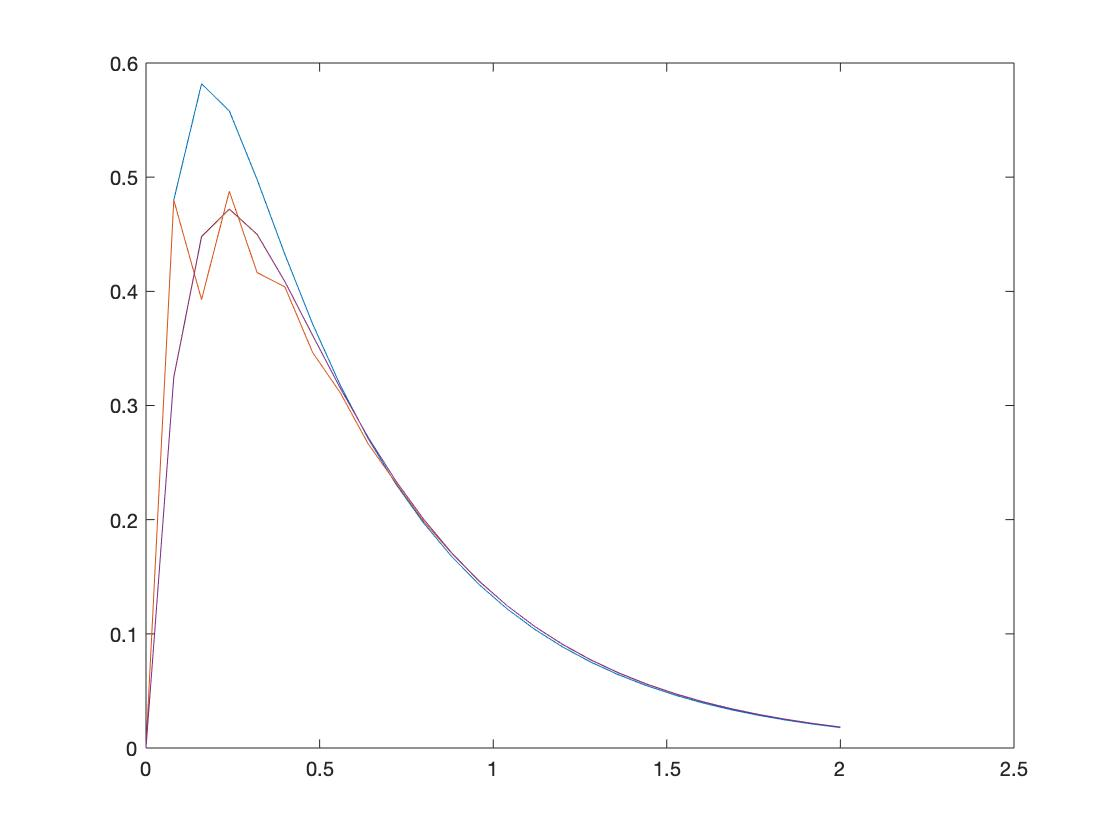
\includegraphics[width=13cm, height=8cm]{Q3.jpg}
\caption{\textbf{Figure 3.1:} Blue: Euler, Orange : AB2, Yellow: RK4, Purple: Exact; \\NOTE that RK4 is very close to the exact solution.}
\end{figure}
\pagebreak
\section*{Question 4}
By Taylor expansion of $y(t_{n+1})$ about $t_{n}$, can see that the Euler method is first-order accurate, the AB2 method is second-order accurate and the RK4 method is fourth-order accurate.
From the graph below can see that as h decreases, the error of RK4 decreases most rapidly, and Euler method converges the slowest , which is consistent with the theory.
\begin{table}[htb]                            
\centering                               
\begin{tabular}{|c|c|c|c|c|}             
\hline                                   
 & h & Euler & AB2 & RK4 \\                      
\hline                                   
0 & 1.6000e-01 & 5.1189e-01 & 5.1189e-01 & 2.1516e-02 \\ 
\hline                                   
1 & 8.0000e-02 & 1.3372e-01 & 5.5368e-02 & 7.6501e-04 \\ 
\hline                                   
2 & 4.0000e-02 & 5.7656e-02 & 1.9884e-04 & 3.6098e-05 \\ 
\hline                                   
3 & 2.0000e-02 & 2.7036e-02 & 1.6996e-04 & 1.9622e-06 \\ 
\hline                                   
4 & 1.0000e-02 & 1.3116e-02 & 6.6197e-05 & 1.1439e-07 \\ 
\hline                                   
5 & 5.0000e-03 & 6.4630e-03 & 1.9560e-05 & 6.9053e-09 \\ 
\hline                                   
6 & 2.5000e-03 & 3.2083e-03 & 5.2614e-06 & 4.2415e-10 \\ 
\hline                                   
7 & 1.2500e-03 & 1.5984e-03 & 1.3612e-06 & 2.6280e-11 \\ 
\hline                                   
8 & 6.2500e-04 & 7.9778e-04 & 3.4600e-07 & 1.6351e-12 \\ 
\hline                                   
9 & 3.1250e-04 & 3.9854e-04 & 8.7210e-08 & 1.0136e-13 \\ 
\hline                                   
10 & 1.5625e-04 & 1.9918e-04 & 2.1891e-08 & 4.9405e-15 \\
\hline                                   
11 & 7.8125e-05 & 9.9567e-05 & 5.4838e-09 & 8.8818e-16 \\
\hline                                   
12 & 3.9063e-05& 4.9778e-05 & 1.3723e-09 & 1.9429e-15 \\
\hline                                   
13 & 1.9531e-05 & 2.4888e-05 & 3.4325e-10 & 2.7756e-16 \\
\hline                                   
14 & 9.7656e-06 & 1.2444e-05 & 8.5842e-11 & 6.7724e-15 \\
\hline                                   
15 & 4.8828e-06 & 6.2217e-06 & 2.1438e-11 & 2.1538e-14\\
\hline                                   
\end{tabular}                            
\caption{}                 
\label{table:MyTableLabel}               
\end{table}                   
\begin{figure}[H]
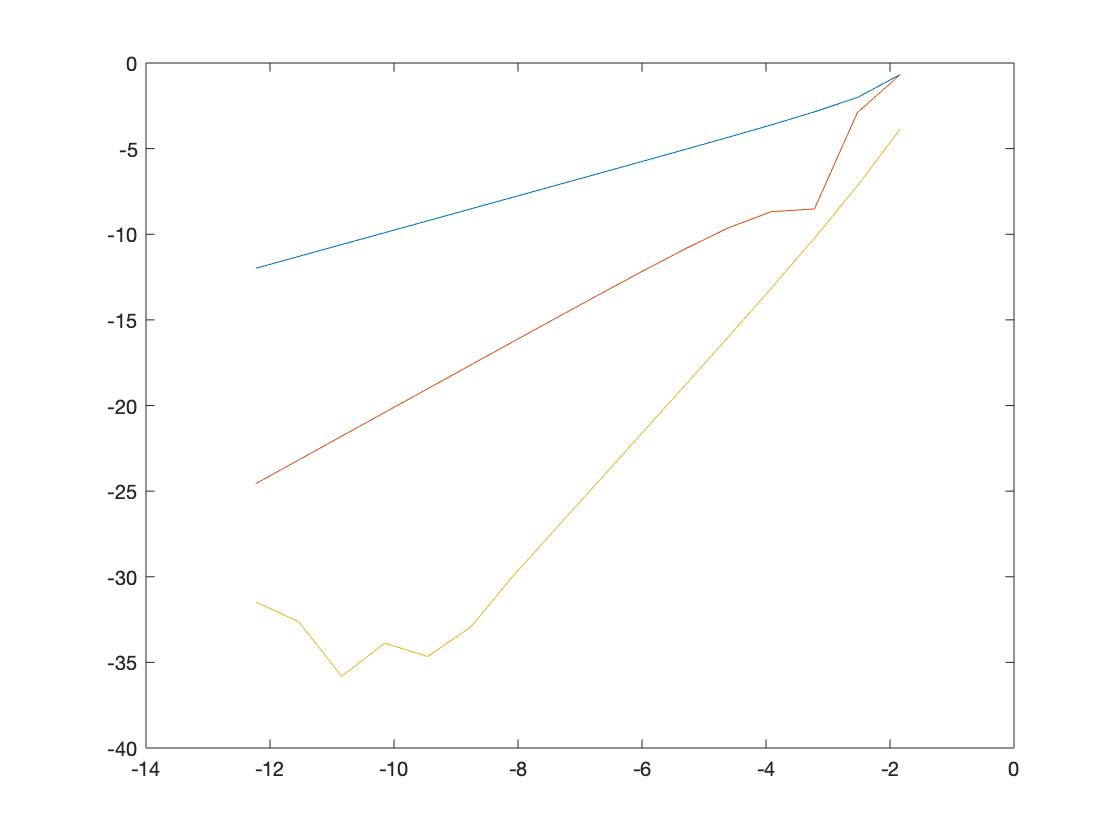
\includegraphics[width=13cm, height=8cm]{Q4.jpg}
\caption{\textbf{Figure 4.1} Blue: Euler, Red: AB2  Yellow: RK4}
\end{figure}
\section*{Question 5}
Substitute $1+x=e^{z}$, we have
$$\diff[2]{y}{z} - \diff{y}{z} + p^{2}y=0$$
Which has solution 
$$y = Ae^{\lambda_{1}z}+Be^{\lambda_{2}z}, for\ p\ \neq \frac{1}{2}.$$
or
$$ y=ze^{\frac{1}{2}x}, for\ p\ = \frac{1}{2};$$
$$\ \lambda_{1,2} = \frac{1 \pm \sqrt{1-4p^{2}}}{2}$$
Substitute initial conditions,
$$A=\frac{1}{\sqrt{1-4p^{2}}},\ B=-\frac{1}{\sqrt{1-4p^{2}}}$$
Hence$$y = \frac{2}{\sqrt{4p^{2}-1}} e^{\frac{\ln(1+x)}{2}}\sin\left(\frac{\sqrt{4p^{2}-1}}{2} \ln(1+x)\right).$$
Consider the eigenvalue problem:
$$\diff[2]{y}{x} + p^{2}(1+x^{2})^{-2}y=0$$
which has general solution:\[y = 
\begin{cases}
\ \ln(1+x)e^{\frac{1}{2}\ln(1+x)}       & p=\frac{1}{2}\\
\ e^{\frac{z}{2}}\left(A\cos\left(\left(\sqrt{p^{2}-\frac{1}{4}}\right)z\right)+B\sin\left(\left(\sqrt{p^{2}-\frac{1}{4}}\right)z\right)\right) & p \neq \frac{1}{2}
\end{cases}\]
For $p\neq \frac{1}{2}$, impose boundary conditions $y(0)=y(1)=0$, $$A=0,
\ \left(\sqrt{p^{2}-\frac{1}{4}}\right)\ln2=k\pi,\ k \in \mathbb{Z}$$
i.e.
$$p^{(k)}=\left(\frac{1}{4}+\left(\frac{k\pi}{\ln2}\right)^{2}\right)^{\frac{1}{2}},\ y^{(k)}(x) = e^{\frac{\ln(1+x)}{2}}\sin\left(\frac{k\pi}{\ln2}\ln(1+x)\right)$$.
And the smallest eigenvalue is $\left(\frac{1}{4}+\left(\frac{\pi}{\ln2}\right)^{2}\right)^{\frac{1}{2}}$.
\pagebreak
\section*{Question 6}
\begin{table}[H]
\caption{Numerical solution at $x_{n}=1$}
    \begin{subtable}{.65\linewidth}
        \caption{p = 4}                       
\begin{tabular}{|c|c|c|c|}        
\hline                            
 & h & $Y_{n}-y_{e}(1)$ & $Y_{n}$ \\                   
\hline                                                                     
1 & 1.0000 & 2.7688e-06 & 0.13576 \\ 
\hline                           
2 & 0.5000 & 1.8295e-07 & 0.13573\\ 
\hline                           
3 & 0.3333 & 1.1707e-08 & 0.13573 \\ 
\hline                           
4 & 0.2500 & 7.3965e-10 & 0.13573 \\ 
\hline                           
5 & 0.2000 & 4.6467e-11 & 0.13573\\ 
\hline                           
6 & 0.1667 & 2.9131e-12 & 0.13573 \\ 
\hline                           
7 & 0.1429 & 1.8247e-13 & 0.13573 \\ 
\hline                           
8 & 0.1250 & 5.5789e-15 & 0.13573 \\ 
\hline                           
9 & 0.1111 & -1.3878e-15 & 0.13573 \\ 
\hline                           
10 & 0.1000& 2.3259e-14 & 0.13573 \\
\hline                           
11 & 0.0909 & 7.9936e-15& 0.13573 \\
\hline                           
12 & 0.0833 &-9.4841e-14 & 0.13573 \\
\hline               
\end{tabular}                     
 \end{subtable}%
    \begin{subtable}{.5\linewidth}
      \caption{p = 5}                   
\begin{tabular}{|c|c|c|c|}       
\hline                           
 & h & $Y_{n}-y_{e}(1)$ & $Y_{n}$\\                  
\hline                                                     
1 & 1.0000  & 9.0854e-06 & 0.085699\\ 
\hline                            
2 & 0.5000  & 5.5948e-07 & -0.085835\\ 
\hline                            
3 & 0.3333  & 3.4554e-08 & -0.085842\\ 
\hline                            
4 & 0.2500  & 2.1444e-09 & -0.085844\\ 
\hline                            
5 & 0.2000  & 1.3351e-10 & -0.085844\\ 
\hline                            
6 & 0.1667 & 8.3292e-12  & -0.085844\\ 
\hline                            
7 & 0.1429  & 5.2086e-13 & -0.085844 \\ 
\hline                            
8 & 0.1250  & 2.8505e-14 & -0.085844\\ 
\hline                            
9 & 0.1111  & -1.5543e-15& -0.085844\\ 
\hline                            
10 & 0.1000 & 1.8138e-14 & -0.085844 \\
\hline                            
11 & 0.0909  & 1.4322e-14 & -0.085844\\
\hline                            
12 & 0.0833  & -6.8986e-14 & -0.085844\\
\hline                                
\end{tabular}                    
\end{subtable} 
\end{table}                   
For p = 5, the method converges much more slowly. The errors decrease as h decreases, which is as expected.
\section*{Question 7}
\begin{table}[H]                            
\centering                               
\begin{tabular}{|c|c|c|c|c|c|c|c|}             
\hline                                   
 1 & 2 & 3 &4 & 5 & 6 & 7 & 8\\                      
\hline 
4.612567 & 4.565358 & 4.560421 & 4.559914 & 
4.559862 & 
4.559857 & 4.559856 & 4.559856 \\
\hline
\end{tabular}                            
\caption{\textbf{Table 7.1}}                 
\label{table:MyTableLabel}               
\end{table}     
Use $h = \frac{1}{12}(\ actually\ 0.1/2^{12})$. For a smaller h, more steps are taken to obtain the numerical solution as the local truncation error is smaller. Hence, the numerical solution is the most accurate with the smallest value of h in the list.
My choice of epsilon is $1 \times 10^{-7}$. I first obtained a numerical solution $p^{*}$ by using binary search with $\mathopen|a-b\mathclose| > 5e-6$ as the condition, then got $\mathopen|\phi(p^{*})\mathclose| \simeq 3.6567e-07$. Hence setting $\epsilon = 1 \times 10^{-8}$ can reach a close solution, which is certainly in the critical region.
\section*{Question 8}
From the physics part in the description of the problem, this is a well-posed problem in p; so there should not be abrupt changes taking place, from ( Figure 8.1 ) below can see that the gradient of function at zero points are much smaller than 1, so it is enough to set $epsilon = 5 \times 10^{-6}$, by Taylor expansion to the first derivative. I obtained numerical solutions with p from 1 to 100, and hence determined the intervals where the zero point lives in by change of sign. Therefore, the first five eigenvalues live in: 12-13, 26-27, 39-40, 53-54, 66-67,  respectively.
After running the program with condition on the width of interval, obtain:
\begin{table}[H]
\centering
\begin{tabular}{|c|c|c|c|c|}  
\hline
$p_{1}$ & $p_{2}$ & $p_{3}$ & $p_{4}$ & $p_{5}$\\
\hline
12.576598 & 26.182779 & 39.711105 & 53.198908 & 66.663298\\
\hline
\end{tabular}
\caption{\textbf{Table 8.1}}
\label{Table}
\end{table}
\begin{figure}[H]
\centering
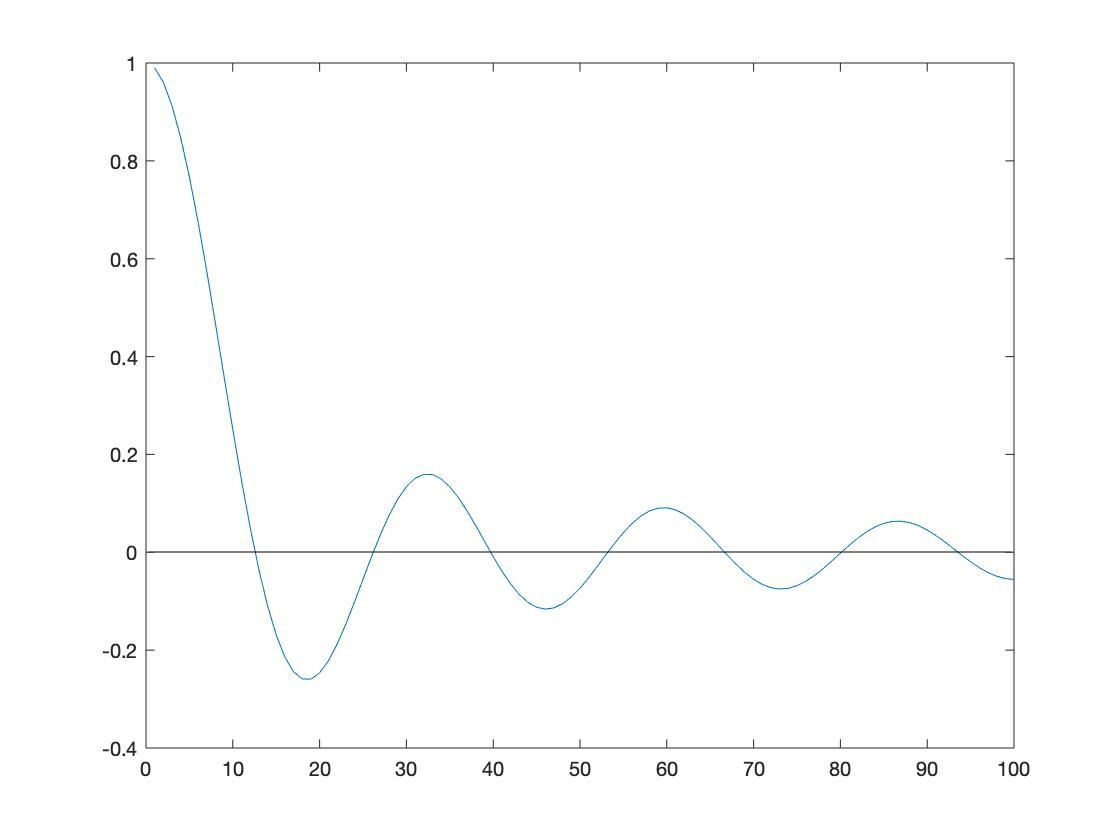
\includegraphics[width = 13cm, height = 8cm]{roots.jpg}
\caption{\textbf{Figure 8.1} }
\end{figure}
\begin{figure}[H]
\centering
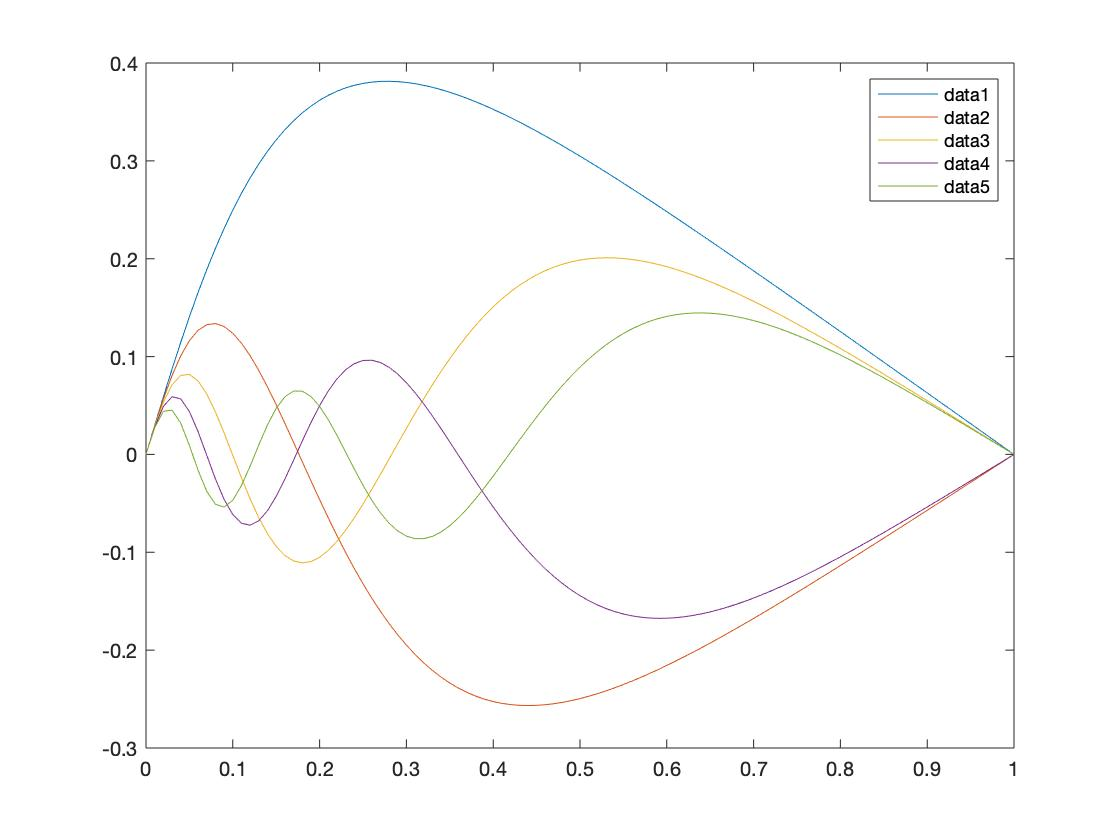
\includegraphics[width = 13cm, height = 8cm]{Q8.jpg}
\caption{\textbf{Figure 8.2} where data(i) is $y^{[i]}$}
\end{figure}
The figure shows that the eigenfunctions have an oscillatory pattern, and they resemble the modes in the solution of wave equations. Physically this is a numerical approximation to small 'normal modes' of an oscillating string. Mathematically, consider WKB approximation, substitute:
$$ y = e^{S(x;\delta)}$$ into (15a), we have, to leading order:
$$\frac{{S}_{0}^{\prime2}}{\delta^{2}}+\frac{2S_{0}^{\prime}S_{1}^{\prime}}{\delta}+\frac{{S}_{0}^{\prime\prime}}{\delta} = -\frac{1}{\delta^2}(1+x)^{-\alpha}$$
as $\delta \to 0$, $$ \frac{{S}_{0}^{\prime2}}{\delta^{2}} \simeq -\frac{1}{\delta^2}(1+x)^{-\alpha}, \frac{2S_{0}^{\prime}S_{1}^{\prime}}{\delta}+\frac{{S}_{0}^{\prime\prime}}{\delta}=0$$ i.e.
$$S_{0}(x) =\pm i\int_{x_{0}}^{x}(1+t)^{-\frac{\alpha}{2}} dt,\ S_{1}(x) = -\frac{1}{4}\ln(-(1+x)^{\alpha}) + C$$
for $\alpha = 10$, $$S_{0}(x) \simeq \pm i\frac{(1+x)^{-4}}{4},\ S_{1}(x) = -\frac{5}{2}\ln(1+x) -e^{i\frac{(2n+1)\pi}{4}} +C$$
Hence: $$ y \approx (1+x)^{-\frac{1}{4}}\left(c_{1}\exp\left(i\left(\frac{(1+x)^{-4}}{4\delta}-\frac{(2n+1)\pi}{4}\right)\right)+c_{2}\exp\left(i\left(-\frac{(1+x)^{-4}}{4\delta}-\frac{(2n+1)\pi}{4}\right)\right)\right)$$
Therefore, after imposing boundary conditions, we can have periodic solutions restricted to [0,1].     
\newpage
\appendix
\section{Programs}
\subsection*{Q1}
\lstinputlisting{Q1.m}
\subsection*{forwardEuler}
\lstinputlisting{forwardEuler.m}
\subsection*{AB2}
\lstinputlisting{AB2.m}
\subsection*{RK4}
\lstinputlisting{RK4.m}
\subsection*{Q6}
\lstinputlisting{Q6.m}
\subsection*{Falseposition}
\lstinputlisting{Falseposition.m}
\subsection*{Command window inputs:}
\lstinputlisting{Q8.m}

\end{document}